%%
%%   TEMPLATE
%%   コピペ用
%%

\documentclass[10pt,b5paper,papersize,dvipdfmx]{jsbook}

%% latexmkを使わない場合
% \usepackage{../sty/vuccaken}
% \usepackage{../sty/vuccaken2019}

%% latexmkならこれでOK
\usepackage{vuccaken}
\usepackage{vuccaken2019}

%% スタイルファイルの読み込みや自作マクロは、
%% 最終的には vuccaken2019.sty の中に書いてください。
%% とりあえずはここに書いてもらって構いません。


\begin{document} % - - - - - - - 以下本文 - - - - - - - - - -

\mokuji{2} % 目次出力

%% - - - - - - - - - - - - - - - - - - - - - - - - %%
\kaishititle%
  {\LaTeX テンプレート(会誌原稿用)}% title
  {テンプレ科学科4回生}% 所属
  {テンプレくん}% name
%% - - - - - - - - - - - - - - - - - - - - - - - - %%

%
\section*{はじめに}
会誌ではjsbookクラスを使います。\par
テーマが複数ある場合は別ファイルで提出してください。

%
\section{セクション}
はじめにこのファイルのソースを自分のtexファイルにコピペしてください。\par
figureのパスには注意してください。


\clearpage
%
\subsection{figure環境}

\begin{figure}[htbp]
  \centering
  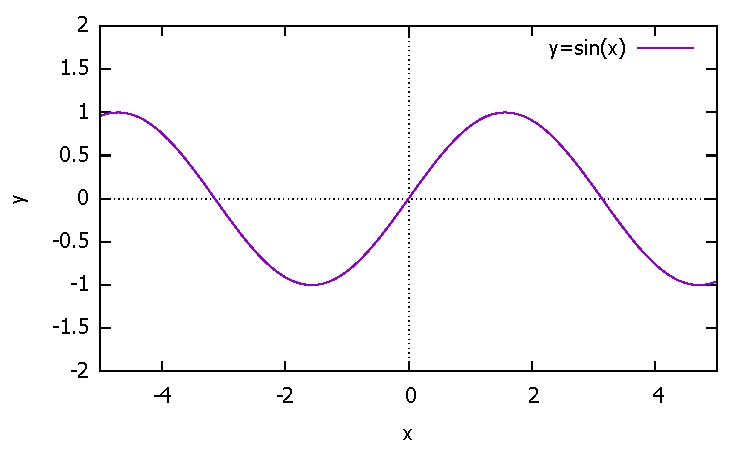
\includegraphics[height=6cm]{temp/fig-sin.pdf}
  \caption{$y=\sin x$のグラフ。gnuplotで作成した。}
  \label{fig:sin}
\end{figure}

図\ref{fig:sin}はイケメンです。

%
\subsection{table環境}

\begin{table}[htbp]
  \centering
  \caption{やさいの表}
  \label{tbl:vegetable}
  \begin{tabular}{r|ccc} \hline
    No. & やさい & いろ & 印象 \\ \hline
    1 & トマト & あかいろ & くさい \\
    2 & キャベツ & みどり & 無味乾燥 \\
    3 & かぼちゃ & きいろ & かたい \\
    4 & にんじん & おれんじ & ゴミ \\ \hline
  \end{tabular}
\end{table}

表\ref{tbl:vegetable}は僕の主観です。


%% 参考文献
\begin{thebibliography}{99}
  \item 著者, 本やページの名前, (URL), 出版社, 出版年.
  \item (複数ある場合は追加)
  \item @vuccaken, 物科研HP, \url{https://vuccaken.github.io}, 2019.
  % \bibitem{キー1} 著者, 本やページの名前, (URL), 出版社, 出版年.
\end{thebibliography}


\end{document} % - - - - - - - - - - - - - - - - - - - - -
%%
%% ファイトだよ!
%%